\thislesson{05 Dicembre 2016}{Campi di funzioni ed Estensioni di mappe razionali}

\section{Campi di funzioni}

Sia $E: y^2=4x^3-ax-b$ una cubica non degenere su $\bbC$.
Siano $x,y:E\rightarrow\bbC$ le funzioni proiezione su $\bbC$, definite sulla cubica.
\begin{definizione}
Indico con $\bbC(t)$ le funzioni razionali in una variabile, quindi $4t^3-ax-b$ è un elemento di $\bbC(t)$, perciò sia $u$ radice quadrata di $f(t)=4t^3-at-b$ e sia $\bbC(t,u)$ l'estensione di $\bbC(t)$ con $u$.\\
Siano inoltre $\bbC(x)$ e con $\bbC(x,y)$ i campi delle funzioni razionali sulle $x$ e $y$ appena definite, che quindi sono funzioni con dominio $E$ e codominio $\bbC$.
\end{definizione}

\begin{osservazione}
Si noti che $\bbC(t)\subseteq\bbC(t,u)$ è un'estensione di grado $2$.\\
Si noti che $\bbC(x)$ è un sottoinsieme delle funzioni razionali di una variabile, calcolate poi in $x$. In particolare è il sottoinsieme delle funzioni razionali in una variabile con denominatore che è non zero se calcolato in $x$, calcolate in $x$. Quindi lo si può pensare come un sottoinsieme delle funzioni razionali non definite in qualche punto.
Analogo per $\bbC(x,y)$.
\end{osservazione}

\begin{proposizione}
$\bbC(x)\cong_{\bbC}\bbC(t)$
\end{proposizione}

\begin{proof}
Considero la mappa $t\mapsto x$ che lascia fisso $\bbC$, si ha che è ben definito poiché l'immagine di una funzione razionale $R(t)$ è una funzione definita tranne in un numero finito di punti, si ha che è surgettivo e omomorfismo di campi, inoltre siccome è non nullo è iniettivo.
\end{proof}

\begin{proposizione}
$\bbC(x,y)\cong_{\bbC}\bbC(t,u)$
\end{proposizione}

\begin{proof}
Considero la mappa $t\mapsto x, u\mapsto y$ che lascia fisso $\bbC$, per vedere che è ben definito bisogna mostrare che se $R(t,u)=S(t,u)$ allora $R(x,y)=S(x,y)$, ma sottraendo mi riduco a mostrare che se $R(t,u)=0$ allora $R(x,y)=0$, ma $R(t,u)$ è $0$ solo se è divisibile per $u^2-f(t)$, ma nell'immagine $y^2-f(x)$ è $0$. Per ESERCIZIO si verifichi che è un omomorfismo e che l'immagine sta dentro $\bbC(x,y)$
\end{proof}

\begin{osservazione}
Si ha che $\bbC(x)\subseteq\bbC(x,y)$ è di grado $2$ quindi gli elementi di $\bbC(x,y)$ si possono rappresentare come $\{ R(x)+y S(x) | R,S \in \bbC(x)\}$.
\end{osservazione}

Ci si chiede se $\bbC(x,y)$ è isomorfo a un certo $\bbC(w)$.
Se lo fosse allora si avrebbe che $x=f(w), y=g(w)$ con $f$ e $g$ razionali, quindi la curva sarebbe parametrizzabile. "Si noti che qui c'è un forte collegamento tra concetti algebrici (campo semplice) e geometrici (parametrizzabilità) (questo si vedrà meglio più avanti nel corso)".

\begin{osservazione}
Non si può usare il teorema dell'elemento primitivo per l'estensione $\bbC\subseteq\bbC(x,y)$ infatti $x$ è trascendente su $\bbC$.
\end{osservazione}

\begin{proposizione}Se la cubica proviene da un toro ( $a=g_2(L), b=g_3(L)$ ) allora $\bbC(x,y)\cong_{\bbC}\bbC(\wp(z),\wp'(z))$.
\end{proposizione}

\begin{proof}
Si noti che quest'ultimo è un campo di funzioni meromorfe, infatti i polinomi nelle $\wp(z)$ e $\wp'(z)$, se non sono nulli, si annullano solo in un numero finito di punti (altrimenti gli zeri hanno un punto di accumulazione). Quindi presi due polinomi $P$ $Q$ calcolati in $\wp(z)$ e $\wp'(z)$ si ha che il loro quoziente $P/Q$ è nullo solo se il denominatore è nullo quindi solo in un numero finito di punti. Per ESERCIZIO si costruisca l'isomorfismo $\bbC[x,y]\rightarrow\bbC[\wp(z),\wp'(z)]$ e poi si passi ai quozienti completando la dimostrazione.
\end{proof}


\section{Estensioni di mappe razionali}
Sia $E'$ un'altra cubica dello stesso tipo di $E$.

\begin{definizione}
Una mappa razionale $E\rightarrow E'$ è una mappa $E\rightarrow E'$ definita su "$\tilde{E}$ meno un numero finito di punti" e che può scrivere in termini razionali di $x$ e $y$, cioè $\varphi(x_0,y_0)=(\varphi_1(x_0,y_0),\varphi_2(x_0,y_0) )$ con $\varphi_1$ e $\varphi_2$ razionali.
\end{definizione}

\begin{osservazione}
Per finire in $E'$ si deve avere che $\varphi_2^2=4\varphi_1^3-a'\varphi_1-b'$, quindi non è facile trovarne nemmeno dalla curva in se stessa. Qualche volta non ce ne sono (a parte le costanti, ovviamente) (vedi quanto scritto sotto per i tori, per aiutarti ad avere un esempio)
\end{osservazione}

Se considero una funzione da un toro in $\bbC$ meromorfa (quindi non definita sul tutto il toro, la chiama così per abbreviare) allora si può estendere ad una funzione olomorfa dal toro verso $\bbP^1(\bbC)$.
Quindi se la curva $E$ proviene da un toro e $E'=\bbC$ posso estendere la mappa razionale a tutta $\tilde{E}$, a valori in $\bbP^1(\bbC)$.
Questo si può fare anche se in arrivo non c'è $\bbC$, ma una qualsiasi $E'$, considerando come codominio della funzione dalla curva estesa $\tilde{E'}$.

\begin{proposizione}
Una mappa razionale $\varphi: E\rightarrow E'$ si estende ad una mappa olomorfa $\tilde{E} \rightarrow \tilde {E'}$.
\end{proposizione}

\begin{proof}
Basta dimostrare che una mappa razionale $\varphi:E\rightarrow \bbC$ si estende a $\tilde{\varphi}:\tilde{E}\rightarrow\bbP^1(\bbC)$ (il caso generale è analogo, ha detto).\\
Ho quindi una mappa da $\tilde{E}$ meno un numero finito di punti a $\bbC$ olomorfa e devo dimostrare che in questi punti NON ha una singolarità essenziale. Siccome i punti mancanti sono in numero finito riesco a trovare per ogni punto un intorno $U$ dove la funzione è definita su tutto $U-\{ p_0\}$ e una carta $\alpha: U\rightarrow \Omega\subseteq\bbC$, in cui suppongo che $\alpha(p_0)=0$ per semplicità. Allora esiste $\psi:\Omega\rightarrow U$ con $\psi(0)=p_0$ tale che $\varphi\circ\psi:\Omega-\{ 0\}\rightarrow \bbC$ è olomorfa. ( $\psi$ è ottenuta come inversa di $\alpha$).\\
Ci basta dimostrare che la mappa $\varphi\circ\psi$ ha al più un polo in $0$.
Supponiamo per assurdo che $0$ sia una singolarità essenziale, allora per il teorema di Weierstrass ogn intorno bucato di $0$ ha immagine densa in $\bbC$. Sia quindi $V_n$ una successione numerabile di dischi aperti bucati di centro zero e raggio $2^{-n}$. Per il Teorema di Baire si ha che l'intersezione delle immagini dei $V_n$ (le mappe olomorfe sono aperte) è un denso, che chiamo $A$.\\
Sia quindi $\xi\in A$, si ha che $\forall\ n \exists\ z_n\in V_n - \{ 0 \} : \varphi ( \psi(z_n ))=\xi$, quindi gli $z_n$ formano una successione tendente a $0$. Ne segue che gli $z_n$ sono almeno una quantità numerabile e siccome $\psi$ è una bigezione anche gli $\psi(z_n)$ sono una quantità almeno numerabile. Ne segue che la fibra $\psi^{-1} (\xi )$ è almeno numerabile, ma ciò è assurdo, poichè $\varphi$ è una mappa razionale (nota che se $\varphi$ è costante non c'è un assurdo, ma sappiamo estendere le mappe costanti). Quindi non ci può essere una singolarità essenziale.
\end{proof}

\notamargine{
Teorema di Baire: In uno spazio metrico completo l'intersezione numerabile di aperti densi è densa.
Oppure: if a non-empty complete metric space is the countable union of closed sets, then one of these closed sets has non-empty interior. (entrambe da Wikipedia) }

\begin{osservazione}
Nota che la dimostrazione fatta vale per qualsiasi curva algebrica che sia una Superficie di Riemann.\\
Nota che l'abbiamo dimostrato in 2 modi, uno usando che le curve ellittiche vengono dai tori (in modo apparentemente semplice, ma che richiede tanta teoria sotto) e uno usando Baire, che è un teorema semplice.\\
Si potrebbe dimostrare in un altro modo puramente algebrico usando che certi anelli di coordinate sono principali, quest'ultima dimostrazione è complicata ma ha il pregio di valere anche in ambiti in cui la caratteristica è un primo $p$.
\end{osservazione}

Come abbiamo già detto è difficile trovare mappe razionali, osserviamo che se due cubiche $E$ e $E'$ provengono da due tori $T$ e $T'$ si ha che ogni mappa razionale $E\rightarrow E'$ induce una mappa olomorfa sui completamenti quindi induce una mappa olomorfa $T\rightarrow T'$. Nota che (come visto alla "lezione del 24 Ottobre") queste mappe sono, a meno di una traslazione, delle moltiplicazioni per costanti, viste su $\bbC$. E che deve valere la relazione tra i reticoli $\mu L\subseteq L'$, condizione molto restrittiva.

\begin{proposizione}
Esiste un algoritmo per dire se esiste una mappa razionale non costante tra due cubiche, se si conoscono stime a priori sul grado della funzione razionale.
\end{proposizione}

\begin{proof} La mappa razionale è una mappa del tipo $(\varphi_1,\varphi_2)$ con $\varphi_i=r_i(x)+y s_i(x)$ $i=1,2$  che deve soddisfare $(r_2(x)+y s_2(x))^2=4(r_1(x)+y s_1(x))^3-a'(r_1(x)+y s_1(x))-b'$, separando i termini in $1$ e $y$ si ricavano due identità nella sola variabile $x$. Qualcosa del tipo $A(x,r_1,r_2,s_1,s_2)=0$ e $B(x,r_1,r_2,s_1,s_2)=0$. Che ci sono algoritmi per capire se questo sistema ha soluzione, se si conoscono delle stime sui gradi.
\end{proof}

\begin{osservazione} Esiste un algoritmo recente per stimare a priori i gradi delle $r_i$ e $s_i$.\\
Esiste un teorema(profondo): Se ne esiste una non costante allora ne esiste una con grado limitato.\\
Nota che le condizioni sui reticoli sono condizioni con quantità trascendenti, difficili da verificare (equivale a chiedersi se delle espressioni che riportano serie infinite (la $\wp$) sono numeri razionali (???))
\end{osservazione}

\thislesson{14 Dicembre 2016}{Le curve ellittiche non sono unirazionali}

\begin{definizione}
Siano $F$ e $L$ due estensioni di un campo $K$. Si dice omomorfismo su $K$ tra $F$ e $L$ una funzione $f:F\rightarrow L$ che sia un omomorfismo e tale che $\forall z\in K\subseteq F$ valga $f(z)=z$.
\end{definizione}
In questa lezione fissiamo $E$ la curva data dall'equazione $y^2=4x^3-g_2x-g_3$ (ed $\widetilde{E}$ la sua chiusura proiettiva).

\notamargine{Abbiamo già visto che una generale curva ellittica si può scrivere in questa forma.}
Consideriamo $\bbC$ come campo base, e consideriamo il campo di funzioni della curva $\bbC(x,y)$. Si noti che l'estensione di campi $\bbC(x)\subseteq\bbC(x,y)$ è algebrica di grado 2.

\begin{definizione}
Una curva si dice razionale se il suo campo di funzioni è isomorfo su $\bbC$ ad un campo del tipo $\bbC(t)$ (con $t$ trascendente su $\bbC$).
\end{definizione}
\begin{definizione}
Una curva si dice unirazionale se il suo campo di funzioni si immerge con un omomorfismo (su $\bbC$) in un campo del tipo $\bbC(t)$ (con $t$ trascendente su $\bbC$).
\end{definizione}
\begin{osservazione}
In $\bbP^2(\bbC)$ le due definizioni sono equivalenti (Teorema di Lüroth).
\end{osservazione}
Supponiamo di voler definire $\varphi: \bbC(x,y) \rightarrow \bbC(t)$ in modo che $\varphi_{|\bbC}$ sia l'identità. Basta definirlo sui generatori: $1\mapsto 1$, $x\mapsto a(t)$ e $y\mapsto b(t)$, dove $a$ e $b$ sono due funzioni razionali di una variabile (ovvero due elementi di $\bbC(t)$).

Affinchè questa mappa sia ben definita deve valere l'uguaglianza (data dall'equazione della curva)   $b(t)^2=4a(t)^3-g_2a(t)-g_3$.
Viceversa, ogni mappa che soddisfa questa identità è un'inclusione $\varphi: \bbC(x,y) \hookrightarrow \bbC(t)$.

Richiedere che $\varphi$ sia un isomorfismo è equivalente a richiedere la sua suriettività, o analogamente che $t\in Im(\varphi)$, ovvero che esista $R\in \bbC(s,r)$ tale che $t=R(a(t),b(t))$.
\begin{osservazione}
La circonferenza ($y^2=1-x^2$) è una curva razionale: la mappa $\varphi$ può essere definita da $\varphi(x)=\frac{2t}{1+t^2}=a(t)$, $\varphi(y)=\frac{1-t^2}{1+t^2}=b(t)$.

In questo modo infatti si ottiene facilmente che $t=\frac{a(t)}{b(t)+1}\in Im(\varphi)$.
\end{osservazione}
\notamargine{In realtà si può mostrare che ogni conica non degenere è razionale.}
\begin{osservazione}
Esistono delle cubiche che sono razionali: ad esempio $y^2=\alpha x^3 + \beta x^2$ può essere parametrizzata come $y=\frac{1-\beta t^2}{\alpha t^3}$ e $x=t\cdot\frac{1-\beta t^2}{\alpha t^3}$.
In questo modo vale $t=\frac{y}{x}$.
\end{osservazione}
\notamargine{Geometricamente questa parametrizzazione si ottiene usando il fascio di rette passante per il punto singolare della cubica.}

L'obiettivo di questa lezione è di mostrare che le curve ellittiche non sono razionali, e nemmeno unirazionali.

\begin{fatto}
Considero $\bbP^1$ come curva in $\bbP^2$. Sia $\varphi$ l'immersione $\bbC(\widetilde{E})\hookrightarrow\bbC(\bbP^1)$ (ovvero l'immersione $\bbC(x,y)\hookrightarrow\bbC(t)$) descritta all'inizio).
Allora esiste una $\varphi^*:\bbP^1\rightarrow\widetilde{E}$ data da $t\mapsto (a(t),b(t))$.
Tale $\varphi^*$ (che sappiamo essere una funzione razionale per definizione) è una funzione olomorfa (solo se si usa $\widetilde{E}$: se uno la considera a valori in $E$ questa proprietà non vale)
\end{fatto}

\begin{teorema}
$\bbC(\widetilde{E})$ non è un campo razionale.
\end{teorema}

\begin{proof}
Supponiamo per assurdo di avere $\psi:\bbC(x,y)\rightarrow\bbC(t)$ isomorfismo (su $\bbC$). Poiché $\psi$ è invertibile si nota che anche $\psi^*$ è invertibile. Si conclude dunque che $\psi^*$ è un biolomorfismo tra $\bbP^1$ e $\widetilde{E}$.

Per ottenere un assurdo è quindi sufficiente mostrare che $\widetilde{E}$ e $\bbP^1$ non sono biolomorfe. Per vedere che non lo sono, consideriamo l'automorfismo di $E$ dato da $(x_0,y_0)\mapsto(x_0,-y_0)$. Questo si estende all'infinito lasciandolo fisso, ed ha tre punti fissi su $E$ (sono solo tre i punti con $y_0=0$). Sappiamo quindi che $\widetilde{E}$ ha un automorfismo con $4$ punti fissi, ma invece $Aut(\bbP^1)=\bbP GL_2(\bbC)$ non contiene nessun elemento con 4 punti fissi (lo abbiamo visto nelle prime lezioni). Segue banalmente che, avendo gruppi di automorfismi diversi, $\widetilde{E}$ e $\bbP^1$ non possono essere biolomorfe e dunque la tesi.
\end{proof}

\begin{osservazione}
Questa dimostrazione si può fare in modo puramente algebrico considerando gli automorfismi dei campi in questione. In particolare l'automorfismo da cui si ricava l'assurdo è $\varphi\in Aut(\bbC(x,y))$ dato da $\varphi(x)=x$, $\varphi(y)=-y$.
\end{osservazione}
%\notamargine{$\psi^*$ si potrebbe definire tra due curve qualsiasi (senza che necessariamente la seconda sia $\bbP^1$), in tal caso la definizione coincide con quella data in questa dimostrazione.} #NONSO...
\begin{lemma}[modello quartico di una cubica]
Una cubica (non singolare) di equazione $y^2=r(z)$ con $deg(r)=3$ è birazionalmente equivalente ad una curva del tipo $y^2=p(x)$ con $deg(p)=4$ e $p$ senza radici doppie.
\end{lemma}
\begin{proof}
Partiamo dal modello quartico $y^2=p(x)$ e arriviamo ad un modello cubico usando solo operazioni birazionali.

Per prima cosa operiamo una traslazione $s=x+\alpha$ per annullare il termine noto di $p(x)$: l'equazione diventa $y^2=sq(s)$.
Operando ora la sostituzione $s=\frac{1}{z}$, ottengo l'equazione $y^2=\frac{q(\frac{1}{z})}{z}$. Moltiplicando l'equazione per $z^4$, e sostituendo $w=z^2y$ si ottiene $w^2=z^3q(\frac{1}{z})=r(z)$, (dove $r(z)$ è un polinomio, perché $deg(q)=3$).

Le operazioni che abbiamo fatto sono birazionali, infatti:
$$z=\frac{1}{x+\alpha}  \;\;\;\;\;\;\;   w=\frac{y}{(x+\alpha)^2}  \;\;\;\leftrightsquigarrow\;\;\;  x=\frac{1}{z}-\alpha   \;\;\;\;\;\;\;  y=\frac{w}{z^2}$$
Resta da verificare solo che $deg(r)=3$ e che $r$ non abbia radici doppie, ma questo segue banalmente dal fatto che $p$ non ha radici doppie (e dunque in particolare $q$ deve avere termine noto $\neq 0$).
\end{proof}

Notiamo che {\it essere unirazionali} per una varietà algebrica è invariante per equivalenza birazionale. Possiamo quindi mostrare che le cubiche non sono unirazionali utilizzando il modello quartico.

\begin{teorema}
Ogni curva ellittica $\widetilde{E}$ non è unirazionale.
\end{teorema}

\begin{proof}[Dimostrazione 1]
Questa dimostrazione utilizza il fatto che $\widetilde{E}$ viene da un toro $\bbC/L$ (che sarà dimostrato più avanti nel corso).

Supponiamo per assurdo che $\widetilde{E}$ sia unirazionale. Allora ho un morfismo $\varphi: \bbC(x,y)\hookrightarrow\bbC(t)$, a cui è associato $\varphi^*:\bbP^1\rightarrow\widetilde{E}$. Poichè $\bbP^1$ è semplicemente connesso, e ho il rivestimento $\pi_L:\bbC\rightarrow\widetilde{E}$, questa mappa si può rialzare a una certa $\phi:\bbP^1\rightarrow\bbC$, ed ottengo dunque un assurdo.

Infatti $\bbP^1$ è compatto, dunque ha immagine limitata, e restringendo $\phi$ a $\bbC\subset\bbP^1$ ho che questa è olomorfa limitata e dunque è costante.
\end{proof}

Vediamo ora una seconda dimostrazione, puramente algebrica, che evita di usare il fatto che ogni curva ellittica è associata ad un toro.
\begin{proof}[Dimostrazione 2]
Utilizziamo il modello quartico della cubica dato dal lemma:

$y^2=(x-\alpha_1)(x-\alpha_2)(x-\alpha_3)(x-\alpha_4)$.

Supponiamo per assurdo di avere soluzioni razionali in un parametro $t$.

Allora $x=\frac{p(t)}{q(t)}$ con $MCD(p,q)=1$.

Sostituendo questa uguaglianza ho che $RHS$ ha denominatore $q(t)^4$ e numeratore coprimo con $q(t)$.
Da questo si ottiene che $y$ deve essere necessariamente $\frac{r(t)}{q(t)^2}$ con $MCD(r,q)=1$.

    \notamargine{L'idea "geometrica" di questa dimostrazione viene dal fatto che le trasformazioni qui descritte corrispondono ad un'isogenia di grado due tra la curva di partenza $\widetilde{E'}$ e quella di arrivo $\widetilde{E}$, e la mappa $\psi^*:\bbP^1\rightarrow\widetilde{E}$ si solleva a una mappa $\bbP^1\rightarrow\widetilde{E'}$ perchè $\bbP^1$ è semplicemente connesso.

    In un certo senso l'analogo algebrico del rivestimento è il passaggio $r^2=abcd\Rightarrow a,b,c,d$ sono tutti quadrati.}

Sostituendo anche questa uguaglianza, e moltiplicando per $q(t)^4$ otteniamo:
$$r(t)^2=(p(t)-\alpha_1q(t))(p(t)-\alpha_2q(t))(p(t)-\alpha_3q(t))(p(t)-\alpha_4q(t))$$
Si osserva facilmente che i polinomi $(p(t)-\alpha_i q(t))$ sono coprimi fra loro: poichè il loro prodotto è un quadrato, allora devono essere tutti quanti dei quadrati. Abbiamo quindi ottenuto che esistono quattro polinomi $r_1$, $r_2$, $r_3$, $r_4$ tali che $(p(t)-\alpha_iq(t))=r_i(t)^2$.

Chiamando $A_i$ l'$i$-esima equazione, considero le equazioni $\alpha_2A_1-\alpha_1A_2$ e $A_1-A_2$.
\begin{eqnarray*}
% \nonumber to remove numbering (before each equation)
  (\alpha_2-\alpha_1)p(t) &=& \alpha_2r_1(t)^2-\alpha_1r_2(t)^2 \\
  (\alpha_2-\alpha_1)q(t) &=& r_1(t)^2-r_2(t)^2
\end{eqnarray*}
Sostituendo i valori di $p(t)$ e di $q(t)$ in $A_3$ e $A_4$ ottengo:
\begin{eqnarray*}
% \nonumber to remove numbering (before each equation)
  (\alpha_2-\alpha_1)r_3^2 &=& (\alpha_2-\alpha_3)r_1^2-(\alpha_1-\alpha_3)r_2^2 \\
  (\alpha_2-\alpha_1)r_4^2 &=& (\alpha_2-\alpha_4)r_1^2-(\alpha_1-\alpha_4)r_2^2
\end{eqnarray*}
Moltiplicando fra loro queste ultime due equazioni si ottiene:
\begin{equation*}
  ((\alpha_2-\alpha_1)r_3r_4)^2 = ((\alpha_2-\alpha_3)r_1^2-(\alpha_1-\alpha_3)r_2^2)((\alpha_2-\alpha_4)r_1^2-(\alpha_1-\alpha_4)r_2^2)
\end{equation*}
Dividendo entrambi i membri per $r_2^4$, e applicando infine le sostituzioni $w=\frac{(\alpha_2-\alpha_1)r_3r_4}{r_2^2}$ e $z=\frac{r_1}{r_2}$, l'equazione diventa:
$$w^2=((\alpha_2-\alpha_3)z^2-(\alpha_1-\alpha_3))((\alpha_2-\alpha_4)z^2-(\alpha_1-\alpha_4))$$
Il polinomio in $z$ al $RHS$ si verifica facilmente non avere radici multiple, quindi rappresenta un'altra cubica.

Inoltre $z=\frac{r_1(t)}{r_2(t)}$, $MCD(r_1,r_2)=1$ e $max(deg(r_1), deg(r_2))\leq\frac{1}{2}\cdot max(deg(p),deg(q))$.

Abbiamo quindi ricavato che da ogni parametrizzazione di una cubica si ricava un'altra parametrizzazione dove $max(deg(p),deg(q))$ è almeno dimezzato.
Procedendo così, poiché il grado iniziale è finito, il procedimento termina ed ho una curva parametrizzata con $max(deg(p),deg(q))=0$.
Tuttavia, questo vuol dire che la curva ha una parametrizzazione non dipendente da $t$, ovvero che l'omomorfismo della definizione $\bbC(x,y)\hookrightarrow\bbC(t)$ manda $x$ in un elemento di $\bbC$, dunque non è iniettivo, e questo ci fornisce un assurdo.
\end{proof}

\chapter{Biliardi ellittici}
\newthought{Introduciamo un altro modo} in cui si ottengono le curve
ellittiche dalle ellissi \notamargine{Abbiamo infatti già visto che si
  possono ottenere come integrali della lunghezza d'arco di un'ellisse}.

Prendiamo un'ellisse di equazione $ax^2 + by^2 = 1$ e supponiamo di
giocare a biliardo sull'ellisse: facendo partire la pallina da un punto
la lanciamo contro il bordo dell'ellisse su cui rimbalza secondo la nota
legge della riflessione \notamargine{Ovvero rispetto alla tangente
  all'ellisse nel punto rimbalza via con lo stesso angolo, come indicato
  in figura}

\begin{center}
  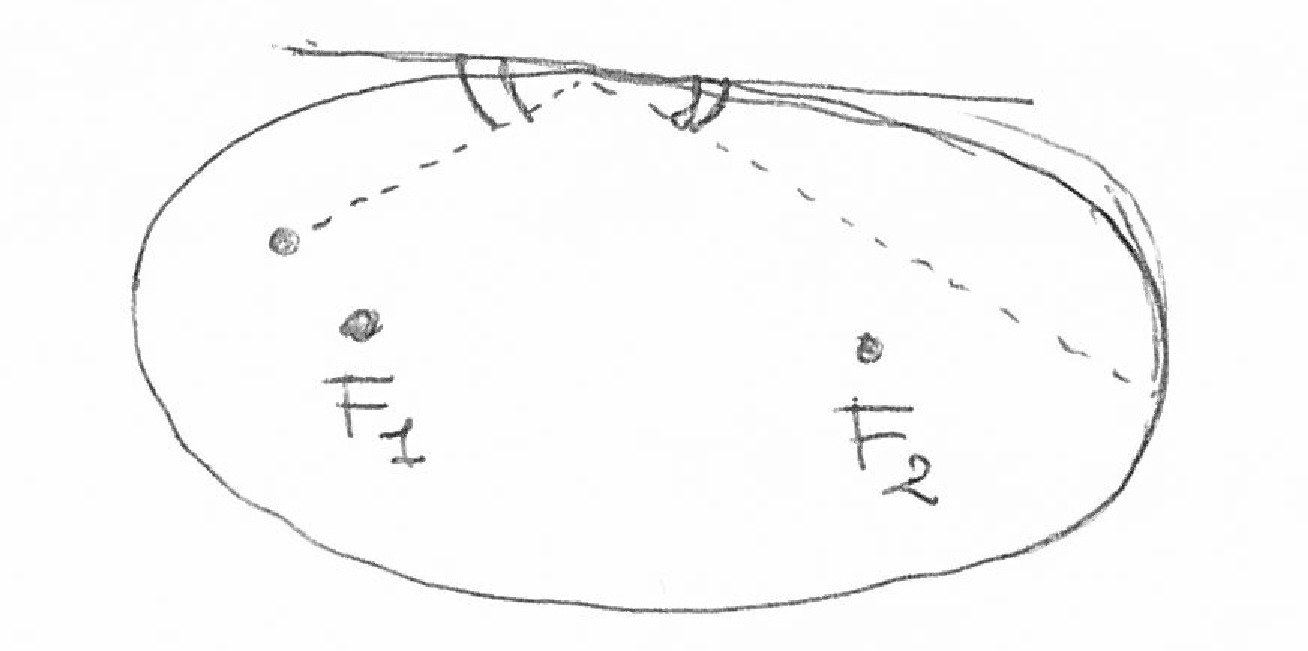
\includegraphics[width=8cm]{lezione-170123-fig1}
\end{center}

Una cosa che è nota da tempo è che le rette che compongono la
traiettoria sono tutte tangenti ad un'altra ellisse ``caustica'' che ha
gli stessi fuochi della prima: abbiamo quindi una famiglia ad un
parametro di ellissi che descrive tutte le possibili traiettorie.

\newthought{Vediamo allora che succede} quando prendiamo un punto $P$
sul bordo dell'ellisse ed una retta $l$ con $P \in l$ e tangente alla
caustica:

Possiamo definire un'applicazione $\phi$ dalle coppie punto-retta in sè
che è la funzione di ``evoluzione'' della traiettoria sul biliardo,
ovvero manda la coppia $(P, l)$ in $(P', l')$ con $P'$ l'altro punto di
intersezione della retta $l$ con l'ellisse e $l'$ la retta passante per
$P'$ che segue la legge della riflessione con $l$.

\notamargine{
  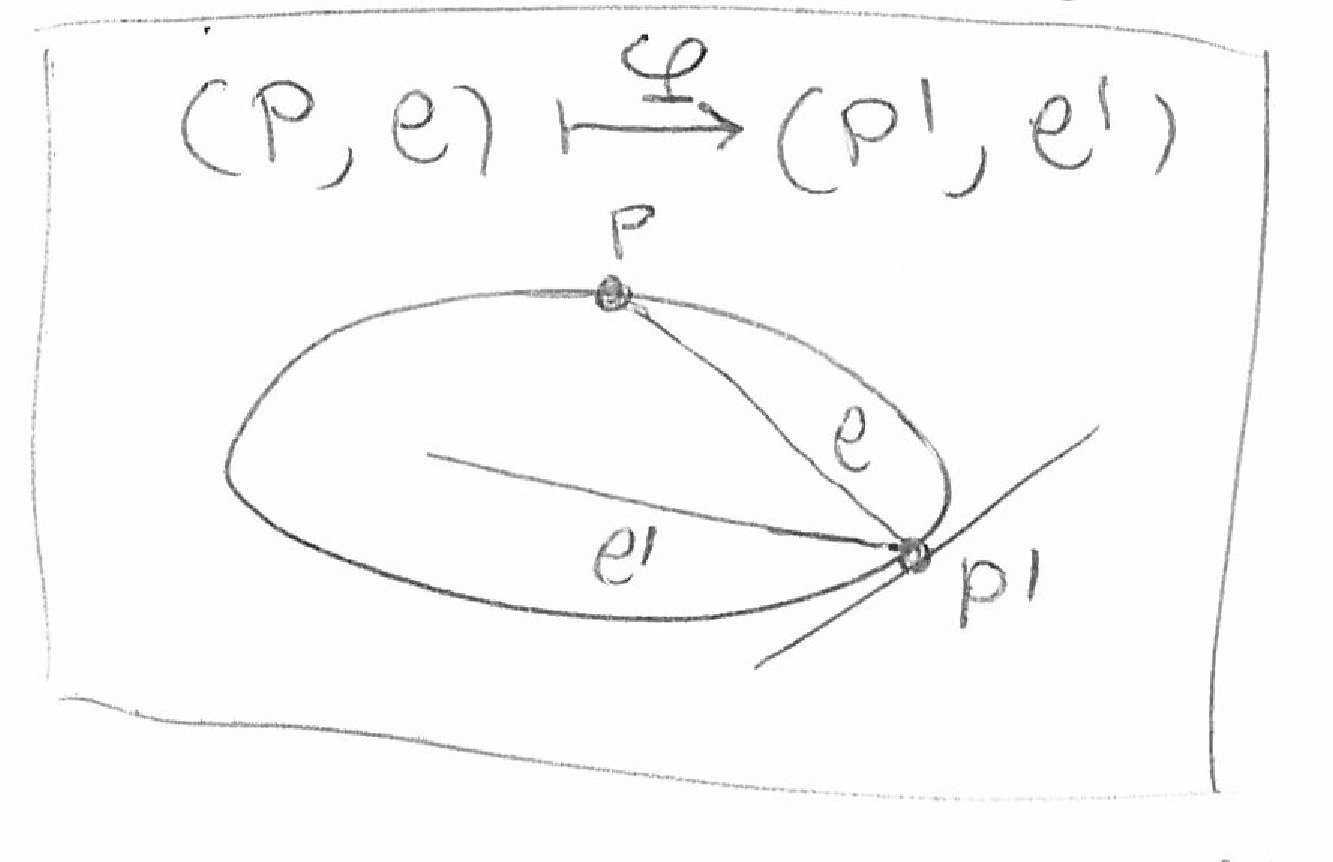
\includegraphics[width=4cm]{lezione-170123-fig2}
}

\newthought{È noto} che le tangenti in $\bbP^2$ ad una conica sono
parametrizzate da un'altra conica: la conica duale.
\notamargine{Tutto ciò non è difficile da verificare: se la conica $\cC$
  ha equazione $f = ax^2 + by^2 + cz^2$ e $(x_0, y_0, z_0) = P \in \cC$
  allora $(\nabla f)_P = (2ax_0, 2by_0, 2cz_0)$ e, ricordando che tutti
  i punti/vettori considerati sono in $\bbP^2$ si ha che dare la retta
  tangente in $P$ è uguale a fornire il vettore $(\nabla f)_P$. D'altra
  parte si riesce ovviamente a recuperare il punto $P$ dato $(\nabla
  f)_P$ a cui è tangente (basta vedere la formula scritta sopra in
  coordinate, visto che i coefficienti della conica sono noti)}
Allora il luogo di punti su cui la $\phi$ agisce è una sottovarietà
(algebrica) di $C_1 \times \hat{C_2}$, con $C_1 = \text{punti della
  conica}$ e $\hat{C_2} = \text{conica duale delle rette tangenti}$.

Il luogo di punti è dato dalle coppie $(P, l) \in C_1 \times \hat{C_2}$
tali che $P \in l$ (che è una condizione chiusa, ovvero dà luogo ad una
sottovarietà algebrica). Questa è anche una superficie di Riemann.

Scrivendo l'equazione si ottiene una curva ellittica e l'operazione
$\phi$ si rivela essere una traslazione sulla cubica detta ``gioco di
Poncelèt''.

Il gioco ``finisce'' se e solo se la traslazione $\phi(x) = x + \tau$ ha
un punto di ordine finito, ovvero $\exists n$
$\phi^n (x) = x + n\tau = x$ se e solo se $n\tau \in L$, il
reticolo. Ovvero si avrebbe $\phi^n(x) = x$ per ogni punto. Allora se il
gioco finisce per una traiettoria finisce per tutte le altre, cosa che
non è per nulla banale.

\notamargine{Come curiosità, se il gioco non finisce, le traiettorie del
  biliardo sono dense nello spazio tra le due ellissi}
